\section{\texorpdfstring{I$^2$C Controller Design}{I2C Controller Design}}
\label{chap:design_i2c_controler}


As explained during the analysis, the I$^2$C controller model of the STM32F405 
microcontroller must be able to recognize the specific sequences of register read and 
write operations (Figures~\ref{fig:i2c_master_transmission} \& Figure~\ref{fig:i2c_master_recv}) that the firmware executes on the real 
hardware to generate the I$^2$C protocol events. This condition must be met for the 
emulated hardware to be able to execute the same I$^2$C events in QEMU.

The analysis shows that the generation of I$^2$C events in the controller model 
depends not only on the current state of the registers but also on the previous I$^2$C 
events. This implies that, in addition to implementing the individual logic for each 
register, a finite state machine (FSM) must be implemented, triggered by the register 
reads and writes.

After an extensive reading of the I$^2$C protocol in the STM32F405 
microcontroller reference manual, and following the sequences of Figures~\ref{fig:i2c_master_transmission} and Figure~\ref{fig:i2c_master_recv} 
which are also shown in the same manual, the state machine of Figure \ref{fig:i2c_fsm} 
was reached. In the Table \ref{tab:i2c_fsm_state} are explained every state.


\begin{figure}[H]
    \centering
    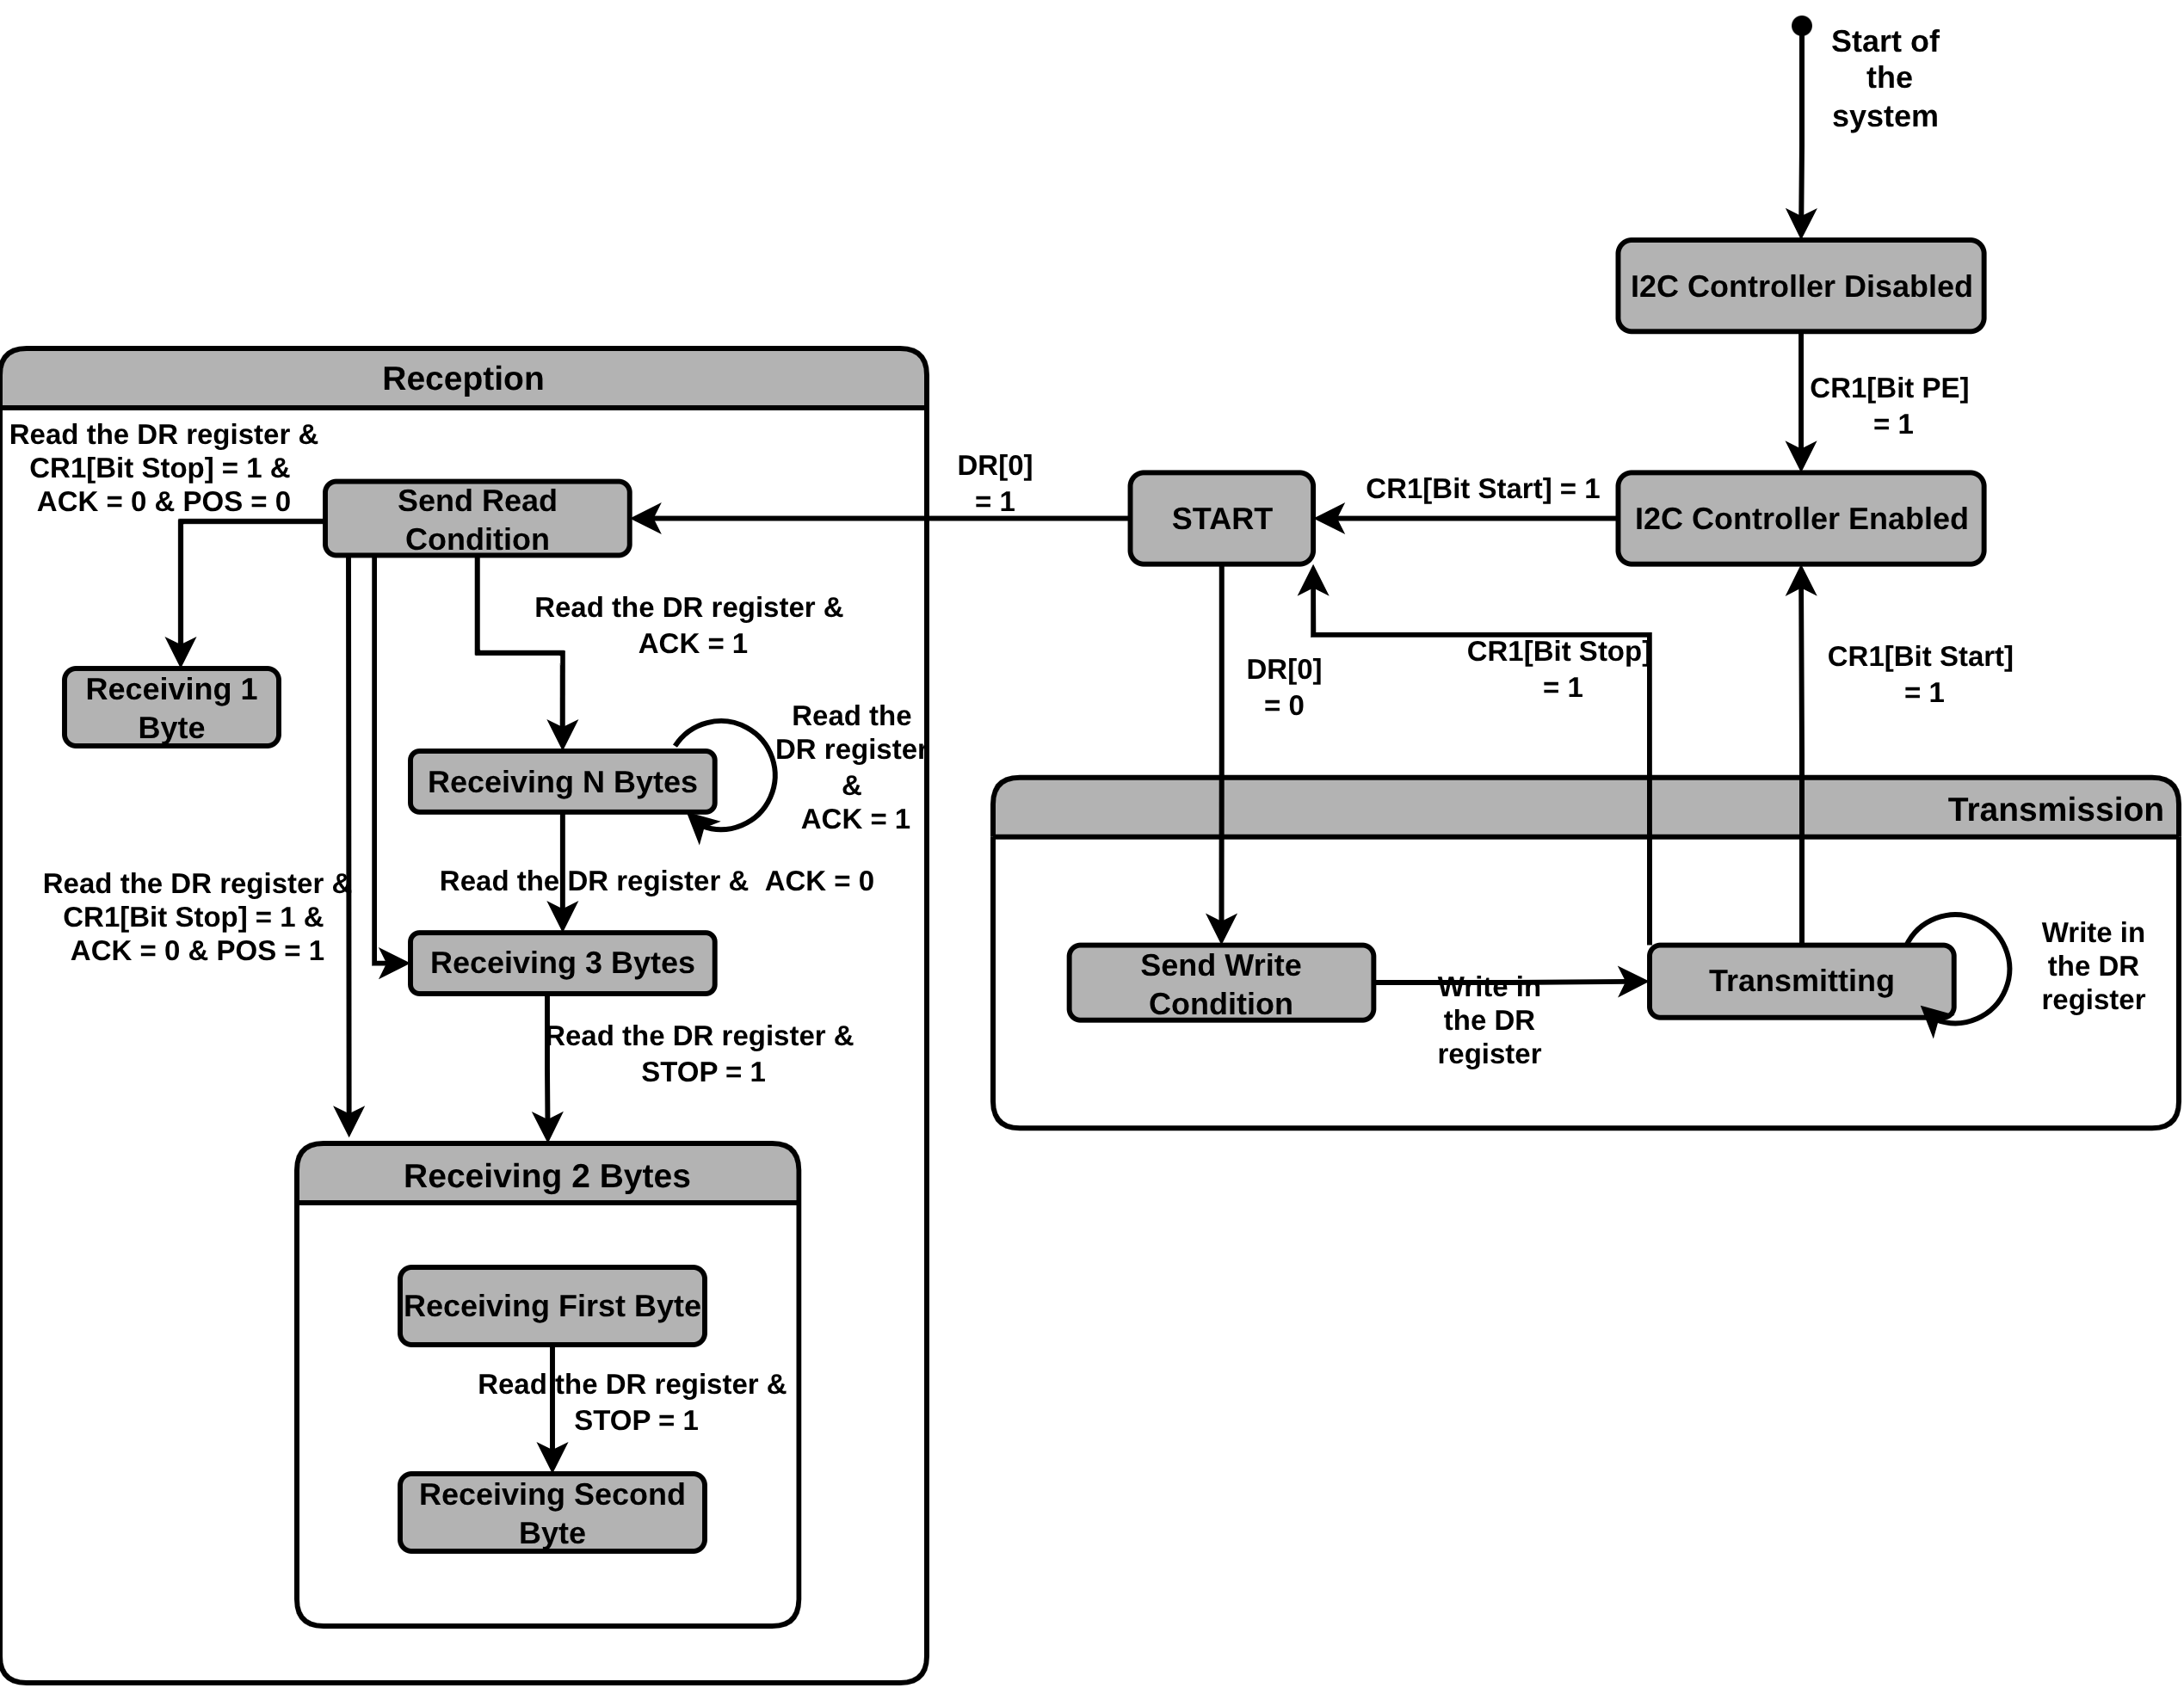
\includegraphics[width=1\textwidth]{Resources/Imagenes/fsm_2.png}
    \caption{stm32f405 i2c controller fsm}
    \label{fig:i2c_fsm}
\end{figure}

\begin{table}[H]
    \small

    \begin{tabularx}{\textwidth}{|c|X|c|X|}
        \hline
        \textbf{Current State}  & \textbf{Transition }  & \textbf{Next State}   & \textbf{Output Action}    \\
                                & \textbf{Condition}    &                       &                           \\
        \hline
        \texttt{DISABLED} & \texttt{CR1[PE] = 1} (Peripheral Enable) & \texttt{IDLE} & Initialize FSM \\
        \hline
        \texttt{IDLE} & \texttt{CR1[START] = 1} & \texttt{START} & Set MSL/BUSY, set SB flag \\
        \hline
        \texttt{START} & \texttt{DR write} (R/W=0) & \texttt{S\_WRITE} & \texttt{i2c\_start\_transfer()}, set ADDR/TXE/BTF \\
        \hline
        \texttt{S\_WRITE} & \texttt{DR write} & \texttt{TRANSMITTING} & \texttt{i2c\_send()}, set TXE/BTF \\
        \hline
        \texttt{TRANSMITTING} & \texttt{DR write} & \texttt{TRANSMITTING} & \texttt{i2c\_send()}, set TXE/BTF \\
        \hline
        \texttt{TRANSMITTING} & \texttt{CR1[START] = 1} & \texttt{START} & Repeated START condition \\
        \hline
        \texttt{TRANSMITTING} & \texttt{CR1[STOP] = 1} & \texttt{IDLE} & \texttt{i2c\_end\_transfer()}, clear flags \\
        \hline
        \texttt{START} & \texttt{DR write} (R/W=1) & \texttt{S\_READ} & \texttt{i2c\_start\_transfer()}, set ADDR/RXNE/BTF \\
        \hline
        \texttt{S\_READ} & \texttt{DR read} \& \texttt{CR1[STOP]=1} \& \texttt{ACK=0} \& \texttt{POS=0} & \texttt{RECV\_1BYTE} & \texttt{i2c\_recv()}, set RXNE/BTF \\
        \hline
        \texttt{S\_READ} & \texttt{DR read} \& \texttt{CR1[STOP]=1} \& \texttt{ACK=0} \& \texttt{POS=1} & \texttt{RECV\_2BYTES\_FIRST} & \texttt{i2c\_recv()}, set RXNE/BTF \\
        \hline
        \texttt{S\_READ} & \texttt{DR read} \& \texttt{ACK=0} \& \texttt{POS=0} & \texttt{RECV\_3BYTES} & \texttt{i2c\_recv()}, set RXNE/BTF \\
        \hline
        \texttt{S\_READ} & \texttt{DR read} \& \texttt{ACK=1} & \texttt{RECV\_NBYTES} & \texttt{i2c\_recv()}, set RXNE/BTF \\
        \hline
        \texttt{RECV\_2BYTES\_FIRST} & \texttt{DR read} \& \texttt{STOP=1} & \texttt{RECV\_2BYTES\_SECOND} & \texttt{i2c\_recv()} (last byte), generate NACK \\
        \hline
        \texttt{RECV\_3BYTES} & \texttt{DR read} \& \texttt{STOP=1} & \texttt{RECV\_2BYTES\_FIRST} & Transition to 2-byte receive mode \\
        \hline
        \texttt{RECV\_NBYTES} & \texttt{DR read} \& \texttt{ACK=1} & \texttt{RECV\_NBYTES} & \texttt{i2c\_recv()}, continue NACK sequence \\
        \hline
        \texttt{RECV\_NBYTES} & \texttt{DR read} \& \texttt{ACK=0} & \texttt{RECV\_3BYTES} & Prepare for 3-byte special case \\
        \hline
        \texttt{RECV\_NBYTES} & \texttt{DR read} \& \texttt{STOP=1} \& \texttt{ACK=0} & \texttt{RECV\_2BYTES\_FIRST} & Final byte handling \\
        \hline
        \texttt{RECV\_1BYTE} & \texttt{STOP=1} & \texttt{IDLE} & \texttt{i2c\_end\_transfer()} \\
        \hline
        \texttt{RECV\_2BYTES\_SECOND} & \texttt{STOP=1} & \texttt{IDLE} & \texttt{i2c\_end\_transfer()} \\
        \hline
    \end{tabularx}



    %\begin{tabular}{|l|p{10cm}|}
    %    \hline
    %    \textbf{State} & \textbf{Description} \\
    %    \hline
    %    DISABLED                & Peripheral disabled (PE bit = 0 in CR1)                       \\
    %    IDLE                    & Peripheral enabled, bus idle, ready to generate START         \\
    %    START                   & START condition generated, waiting for address transmission   \\
    %    SENT\_WRITE             & Address transmitted in write mode, waiting for data or register 
    %                                address \\
    %    SENT\_READ              & Address transmitted in read mode, configuring receive mode    \\
    %    TRANSMITTING            & Actively transmitting data bytes to slave device              \\
    %    RECV\_1BYTE             & Single-byte read mode configured (NACK pre-loaded)            \\
    %    RECV\_2BYTES\_FIRST     & Two-byte read, first byte reception                           \\
    %    RECV\_2BYTES\_SECOND    & Two-byte read, second byte reception                          \\
    %    RECV\_3BYTES            & Three-byte read mode (special NACK timing)                    \\
    %    RECV\_NBYTES            & Multi-byte read mode (N $>$ 3, ACK enabled)                   \\
    %    \hline
    %\end{tabular}

    \caption{STM32F4 I2C Master Mode Finite State Machine Transitions}
    \label{tab:i2c_fsm_state}
\end{table}